\documentclass[conference]{IEEEtran}
\IEEEoverridecommandlockouts
% The preceding line is only needed to identify funding in the first footnote. If that is unneeded, please comment it out.
%Template version as of 6/27/2024

\usepackage{cite}
\usepackage{amsmath,amssymb,amsfonts}
\usepackage{algorithmic}
\usepackage{graphicx}
\usepackage{textcomp}
\usepackage{xcolor}
\usepackage{float} % Para controle de posição de figuras/tabelas
\usepackage{multirow} % Para tabelas com múltiplas linhas
\usepackage{booktabs} % Para melhor aparência de tabelas (opcional)
\usepackage{subcaption}

% Definição do BibTeX style
\bibliographystyle{IEEEtran}
\def\BibTeX{{\rm B\kern-.05em{\sc i\kern-.025em b}\kern-.08em
    T\kern-.1667em\lower.7ex\hbox{E}\kern-.125emX}}
\begin{document}

\title{IMAGE-BASED GIMBAL CONTROL FOR OBJECT TRACKING\\
{\footnotesize}
\thanks{Marcos Maximo is partially funded by CNPq - National Research Council of Brazil through the grant 307525/2022-8.}
}

%\author{\IEEEauthorblockN{1\textsuperscript{st} Given Name Surname}
%\IEEEauthorblockA{\textit{dept. name of organization (of Aff.)} \\
%\textit{name of organization (of Aff.)}\\
%City, Country \\
%email address or ORCID}
%\and
%\IEEEauthorblockN{2\textsuperscript{nd} Given Name Surname}
%\IEEEauthorblockA{\textit{dept. name of organization (of Aff.)} \\
%\textit{name of organization (of Aff.)}\\
%City, Country \\
%email address or ORCID}
%\and
%\IEEEauthorblockN{3\textsuperscript{rd} Given Name Surname}
%\IEEEauthorblockA{\textit{dept. name of organization (of Aff.)} \\
%\textit{name of organization (of Aff.)}\\
%City, Country \\
%email address or ORCID}
%}
\author{\IEEEauthorblockN{Lucas Ávila Silva}
\IEEEauthorblockA{\textit{Division of Aeronautics Engineering (IEA)} \\
\textit{Instituto Tecnológico de Aeronáutica}\\
São José dos Campos, Brazil \\
lucas.avilas@outlook.com}
\and
\IEEEauthorblockN{Marcos R. O. A. Máximo}
\IEEEauthorblockA{\textit{Computer Science Division (IEC)} \\
\textit{Instituto Tecnológico de Aeronáutica}\\
São José dos Campos, Brazil \\
maximo.marcos@gmail.com}
\and
\IEEEauthorblockN{Raphael das Neves Calvo}
\IEEEauthorblockA{\textit{Flight Control Systems (GIS)} \\
\textit{Embraer S.A.}\\
São José dos Campos, Brazil \\
raphael.calvo@embraer.com.br}
}

\maketitle

\begin{abstract}
The capability for real-time object detection and tracking has become fundamental for autonomous and security systems. Integrating this technology with multi-axis gimbal systems significantly elevates performance, providing image stabilization and precise tracking. This work proposes the development of a comprehensive and robust control solution for object tracking in real-time acquired images using a two-degree-of-freedom (2-DOF) gimbal platform. The contributions include an integrated system architecture uniting visual perception (YOLOv8), data communication, and motion control. The system model modularly incorporates critical nonlinearities such as Coulomb friction and the combined controller and actuator delay. Validation through real-time simulation, considering a total application latency of 124 ms, demonstrates the viability of a stable and responsive platform. The developed PID control system was capable of stabilizing the gimbal's rotational axes, effectively tracking the zero reference (image center) with a settling time of approximately 5 s.
\end{abstract}

\begin{IEEEkeywords}
Object Detection, Tracking, YOLO, Gimbal Control, Communication Delay, PID Control.
\end{IEEEkeywords}

\section{INTRODUCTION}
The ability to detect and track objects in real-time is crucial for autonomous and security systems, spanning from industrial production and autonomous vehicles to sophisticated military operations. When paired with multi-axis gimbal systems, this technology overcomes the field-of-view limitations of fixed sensors, providing image stabilization and precise Line-of-Sight (LOS) reorientation for monitoring distant or fast-moving targets \cite{GimbalYOLO}. In the aeronautical sector, gimbals equipped with optoelectronic sensors are core components of Intelligence, Surveillance, and Reconnaissance (ISR) systems in Unmanned Aerial Vehicles (UAVs).

Despite significant advancements, developing robust and high-performance visual tracking systems faces considerable challenges. Control precision is often hindered by the inherent complexity of gimbal dynamics, which includes nonlinearities (such as friction) \cite{espinosa2016diseno} and the communication delays intrinsic to distributed system architectures \cite{TONG2020105312, KIESEL2022238}. 

While computer vision has seen great success with algorithms like YOLO \cite{YOLO}, R-CNN \cite{6909475}, Faster R-CNN \cite{7485869}, and SSD \cite{Liu_2016}, the integration of these heavy computational loads into real-time control loops remains non-trivial. The foundational mathematics of deep learning, as described by Goodfellow et al. \cite{Goodfellow-et-al-2016} and Brunton and Kutz \cite{Brunton_Kutz_2022}, highlights the trade-off between accuracy and inference speed.

Furthermore, control literature has explored advanced techniques like Sliding Mode Control (SMC) \cite{Rahmat2016Sliding} and Fuzzy Logic Control (FLC) \cite{Galal2009Fuzzy} for turret and gimbal systems. However, few works integrate a complete, end-to-end architecture while rigorously modeling both the mechanical nonlinearities and the communication delays present in real-world closed-loop systems using recent state-of-the-art detection algorithms like YOLOv8 \cite{Jocher_Ultralytics_YOLO_2023}.

In this context, this work presents a comprehensive control solution for image-based object tracking utilizing a two-degrees-of-freedom (2-DOF) gimbal platform. The objective is to develop a control strategy capable of adjusting the platform's orientation in real-time to keep the object of interest centralized within the image field of view.

The main contributions of this study are:
\begin{itemize}
    \item The proposition of an integrated and complete system architecture uniting visual perception (YOLOv8), Kalman filtering \cite{Kalman1st}, and PID motion control with the detailed electromechanical dynamics of a 2-DOF gimbal.
    \item The validation of the control system via real-time simulation, demonstrating a stable and responsive platform for object tracking under conditions emulating operational latency.
\end{itemize}

The remainder of this paper is organized as follows. Section II details the system architecture and mathematical modeling. Section III presents the control design and state estimation. Section IV provides the experimental results and discussion. Finally, Section V concludes the work and outlines future research directions.

\section{SYSTEM ARCHITECTURE AND MODELING}
The proposed solution integrates computer vision, state estimation, and motion control, applied to a two-degrees-of-freedom (2-DOF) gimbal platform. The overall system architecture, illustrated in Fig.~\ref{arquiteturaprojeto}, operates in a closed loop, where the image coordinates from the sensor serve as feedback for the gimbal's control mechanism.

\begin{figure}[!t]
    \centering
    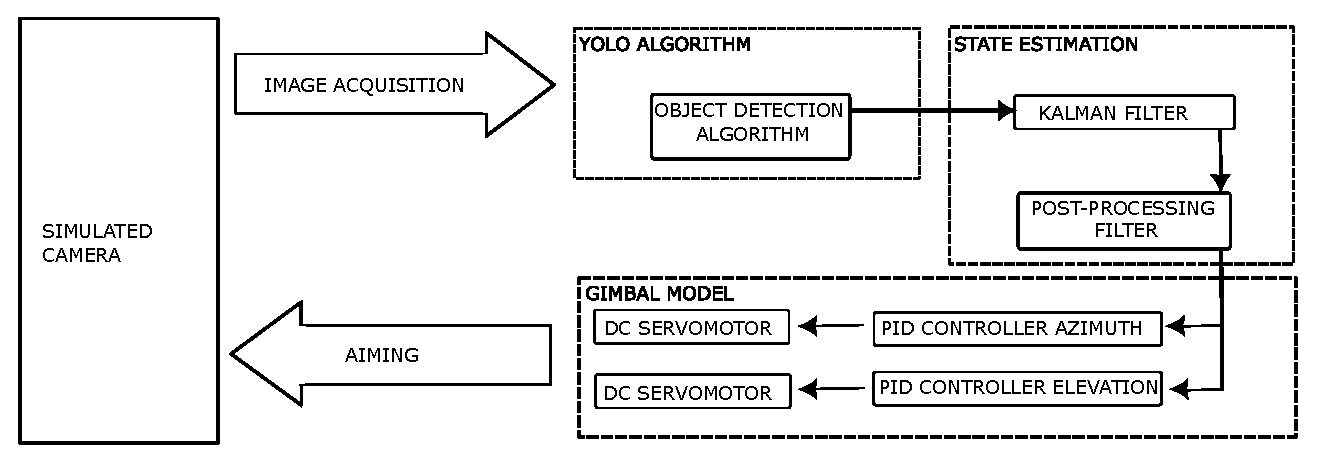
\includegraphics[width=\columnwidth]{images/arquitetura-eps-FINAL.eps}
    \caption{Proposed end-to-end system architecture for image-based object tracking.}
    \label{arquiteturaprojeto}
\end{figure}

\subsection{Image-Based Sensing}
The vision system utilizes the YOLOv8 algorithm \cite{Jocher_Ultralytics_YOLO_2023}, implemented using the Ultralytics framework, to process input image frames ($1280 \times 720$ pixels) and output the bounding box coordinates of the detected object. This raw data is transmitted to the Simulink control environment via the User Datagram Protocol (UDP), chosen for its low-latency characteristics required for real-time streaming \cite{gatimu2020experimental}.

\subsection{Gimbal Dynamics and Actuator Modeling}
The 2-DOF gimbal model, reduced to azimuth and elevation axes, forms the core of the mechatronic system. To ensure realism, the model incorporates the dynamics of the DC servomotors and critical nonlinearities.

\subsubsection{Rotational Axes Dynamics}
Adopting the simplifications of neglecting cross-coupling effects, the rotational dynamics for the inner (elevation, $I$) and outer (azimuth, $O$) gimbals, including the combined viscous friction $k_{vf}$, are simplified to a linear function with friction modeled as a disturbance. For the inner gimbal, the required motor torque ($T_{m_I}$) is given by:
\begin{equation}
    \label{eq:torque_inner}
    T_{m_I} = I^I_y \alpha_{IB_y} + k_{vf}\Omega_{IB_y}, 
\end{equation}
where $I^I_y$ is the moment of inertia about the y-axis, $\alpha_{IB_y}$ is the angular acceleration, and $\Omega_{IB_y}$ is the angular velocity. The same form is used for the outer gimbal, substituting the respective inertial parameters. The inertial parameters used in the model are shown in Table~\ref{tabelaparametrogimbal}.

\begin{table}[!t]
\caption{Gimbal's Inertial Parameters \cite{espinosa2016diseno}.}
\label{tabelaparametrogimbal}
\centering
\begin{tabular}{|c||c|} 
    \hline
    \textbf{Parameter} & \textbf{Value} \\ [0.5ex] 
    \hline\hline
    $I^I_x$ & $1.68 \times 10^{-4} \, (\text{kg} \cdot \text{m}^2)$\\ 
    \hline
    $I^I_y$ & $1.78 \times 10^{-4} \, (\text{kg} \cdot \text{m}^2)$ \\
    \hline
    $I^I_z$ & $1.16 \times 10^{-4} \, (\text{kg} \cdot \text{m}^2)$ \\
    \hline
    $I^O_x$ & $2.62 \times 10^{-3} \, (\text{kg} \cdot \text{m}^2)$ \\
    \hline
    $I^O_y$ & $2.47 \times 10^{-3} \, (\text{kg} \cdot \text{m}^2)$ \\
    \hline
    $I^O_z$ & $4.66 \times 10^{-4} \, (\text{kg} \cdot \text{m}^2)$ \\
    \hline
\end{tabular}
\end{table}

\subsubsection{DC Motor Transfer Function}
The motors are modeled using the equivalent circuit diagram, considering armature resistance ($R_a$), inductance ($L_a$), counter electromotive force ($K_e$), and torque constant ($C_m$). Combining the electrical and mechanical equations, the transfer function relating the input voltage $U(s)$ to the motor torque $T_m(s)$ is derived as:
\begin{equation}
\label{eq:FT_motor_torque}
\frac{T_{m}(s)}{U(s)} = \frac{C_m (I s + k_{vf})}{L_a I s^2 + (R_a I + L_a k_{vf})s + (R_a k_{vf} + C_m K_e)},
\end{equation}
where $I$ is the total moment of inertia (gimbal + motor + encoder) for the respective axis.

\subsection{Communication Delay Modeling}
The system's real-time performance is heavily influenced by latency. The total application-perceived latency ($\Delta \tau_{l,\text{application}}$) is defined as the sum of sensor processing, network transmission, controller processing, and actuator response delays \cite{KIESEL2022238}. The combined controller and actuator delay is estimated at $\tau = 40 \text{ ms}$. This pure time delay ($e^{-s\tau}$) is approximated using a $2^{nd}$ order Padé approximation to integrate its effect on the system stability analysis:
\begin{equation}
e^{-s\tau} \approx \frac{1 - s\tau/2 + s^2\tau^2/12}{1 + s\tau/2 + s^2\tau^2/12}. 
\end{equation}
The resultant total application latency, encompassing $\tau_{\text{sensor}} \approx 60 \text{ ms}$ (YOLO processing) and $\tau_{\text{network}} \approx 24 \text{ ms}$ (UDP), is $\Delta \tau_{l,\text{application}} \approx 124 \text{ ms}$ for the simulation environment.

\section{CONTROL AND STATE ESTIMATION}

\subsection{State Estimation and Pre-processing}
The raw 2D position coordinates ($x, y$) obtained from the YOLOv8 algorithm are prone to noise. To mitigate these effects, a Kalman Filter is employed for state estimation, providing a smooth and refined trajectory of the target. This approach overcomes the limitations of other methods \cite{Kalmanxalpha}. Although advanced nonlinear estimators exist, the linear Kalman Filter proved sufficient for this application.

\subsubsection{Kalman Filter Design}
The filter is designed to track the object's 2D position and velocity, with a state vector $\hat{\mathbf{x}} = [x, y, \dot{x}, \dot{y}]^T$. The state transition matrix ($A$) models constant velocity, and the measurement matrix ($C$) only observes the position:
\begin{equation*}
A = \begin{pmatrix} 1 & 0 & T & 0 \\ 0 & 1 & 0 & T \\ 0 & 0 & 1 & 0 \\ 0 & 0 & 0 & 1 \end{pmatrix}, \quad C = \begin{pmatrix} 1 & 0 & 0 & 0 \\ 0 & 1 & 0 & 0 \end{pmatrix}.
\end{equation*}
A conservatively high standard deviation for the camera noise ($\sigma_{cam} = 1000 \text{ pixels}$) was deliberately selected for the Measurement Noise Covariance ($R$). This choice prioritizes the internal constant-velocity model predictions over the instantaneous YOLOv8 measurements, effectively smoothing the tracking signal. Low values of $\sigma_{cam}$ were found to couple the high-frequency jitter inherent in bounding box detections into the control loop, resulting in noisy control inputs and undesirable actuator oscillation.

\subsubsection{Post-Processing and Angular Conversion}
The smoothed coordinates are converted from pixels to angular displacements (Elevation ($\epsilon$) and Azimuth ($\eta$)) relative to the camera's principal axis using the pinhole model:
\begin{equation}
    \eta_{\text{Displacement}} = \arctan\left(\frac{x - c_x}{f_x}\right)
\end{equation}
\begin{equation}
    \epsilon_{\text{Displacement}} = \arctan\left(\frac{y - c_y}{f_y}\right)
\end{equation}
where $(c_x, c_y)$ are the principal point coordinates, and $(f_x, f_y)$ are the camera's focal point coordinates. These angular displacements serve as the error signal for the motion controllers, targeting the zero reference.

\subsection{PID Control Design}
A Proportional-Integral-Derivative (PID) controller ($C(s) = K_p + \frac{K_i}{s} + K_d s$) was selected. The gains were initially determined using the Root Locus technique and refined via the $\texttt{pidtune()}$ function in MATLAB to optimize performance specifications. The final parameters used for the two rotational axes are presented in Table~\ref{PID parameters table}.

\begin{table}[!b]
\caption{PID Controller Parameters.}
\label{PID parameters table}
\centering
\begin{tabular}{|c||c|c|} 
    \hline
    \textbf{Parameter} & \textbf{Elevation Axis ($I$)} & \textbf{Azimuth Axis ($O$)} \\ [0.5ex] 
    \hline\hline
    $K_p$ & $1$ & $1$ \\ 
    \hline
    $K_i$ & $0.15$ & $0.2$ \\
    \hline
    $K_d$ & $0.5$ & $0.45$ \\
    \hline
\end{tabular}
\end{table}

\section{RESULTS AND DISCUSSION}
This section presents a detailed evaluation of the system's performance, encompassing object detection metrics, latency characterization, and the tracking response of the closed-loop system. The simulations were performed on a high-performance computer equipped with an Intel Core i7-13650HX processor, 16 GB of RAM, and an Nvidia GeForce RTX 4050 GPU, ensuring that the computational resources were sufficient for the simulation processing. A visual result of the simulation running is shown in Figure~\ref{simulacao}. A video demonstration of the real-time simulation performance is available online\footnote{https://www.youtube.com/watch?v=ZxFmtXqEOyg}. 

\begin{figure}[!t]
\centering
    \begin{subfigure}{0.2\textwidth}
        \centering
        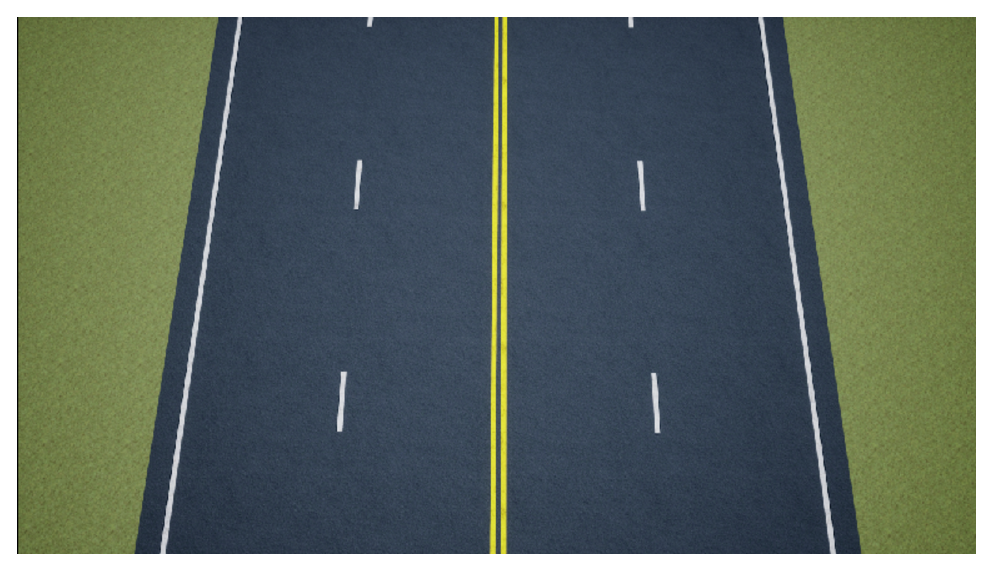
\includegraphics[width=1\linewidth]{images/Car3.eps}
    \end{subfigure}
    \begin{subfigure}{0.2\textwidth}
        \centering
        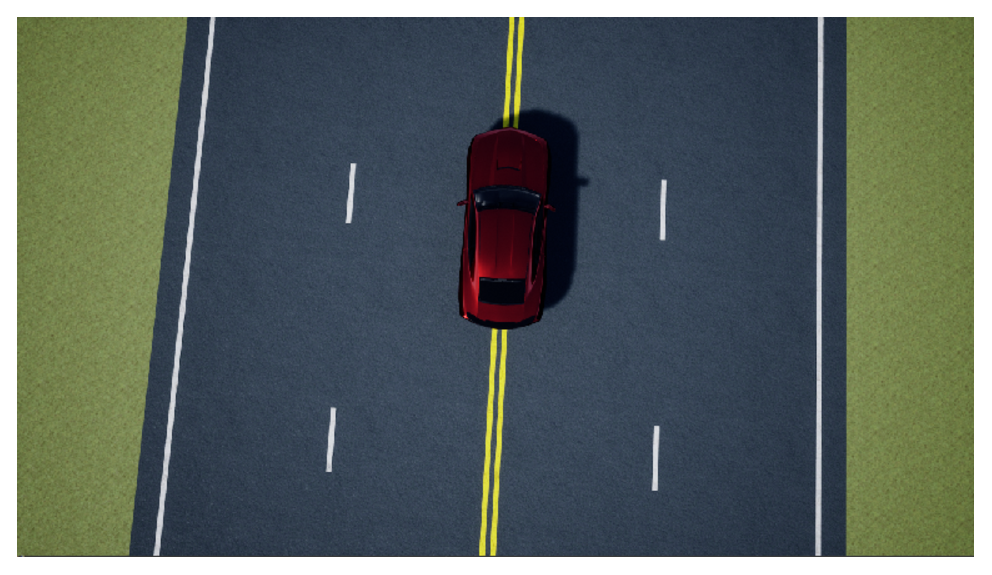
\includegraphics[width=1\linewidth]{images/CAR1.eps}
    \end{subfigure}
    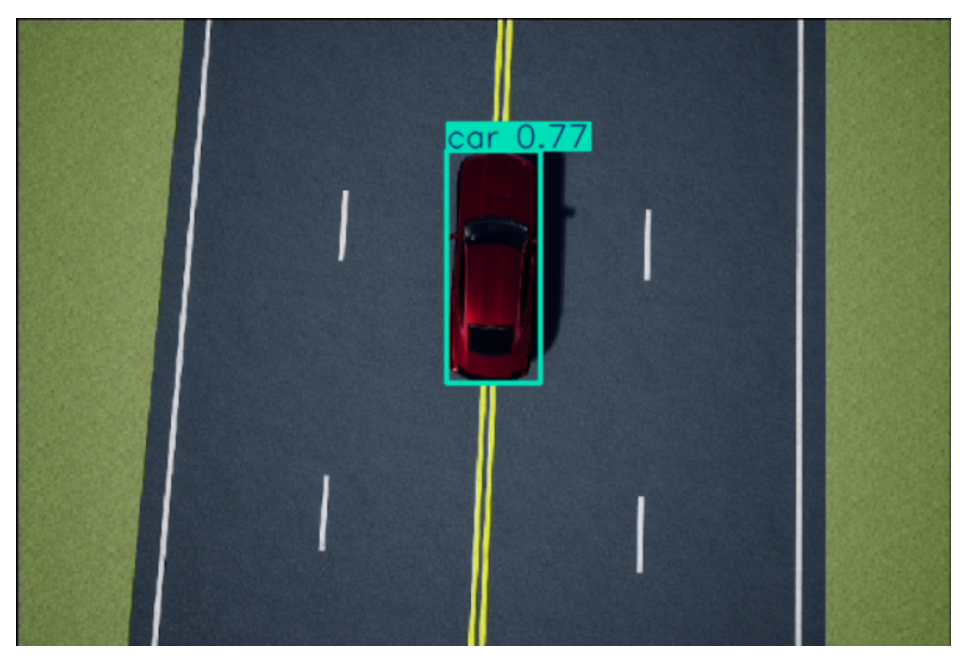
\includegraphics[width=0.5\columnwidth]{images/car2.eps}
    \caption{Results obtained from simulation in 3D environment.}
    \label{simulacao}
\end{figure}

\subsection{Object Detection Performance}
The YOLOv8 algorithm was trained using the VisDrone2019 dataset \cite{VisDrone}, which contains 288 video clips and over 10,000 static images captured by drone-mounted cameras. This dataset was selected due to its wide range of environments and object densities, presenting a realistic challenge for the vision system.

The training process followed the Ultralytics documentation \cite{YOLOTraining}. Fig.~\ref{mAPssistema} illustrates the evolution of the Mean Average Precision (mAP) during training. While the analysis of the loss function convergence, shown in Fig.~\ref{Lossfcn}, indicates stable learning and the absence of significant overtraining, the overall performance metrics reveal challenges inherent to the dataset.

\begin{figure}[!t]
    \centering
    \begin{subfigure}{0.2\textwidth}
        \centering
        \includegraphics[width=1\linewidth]{images/mAP50.eps}
    \end{subfigure}
    \begin{subfigure}{0.2\textwidth}
        \centering
        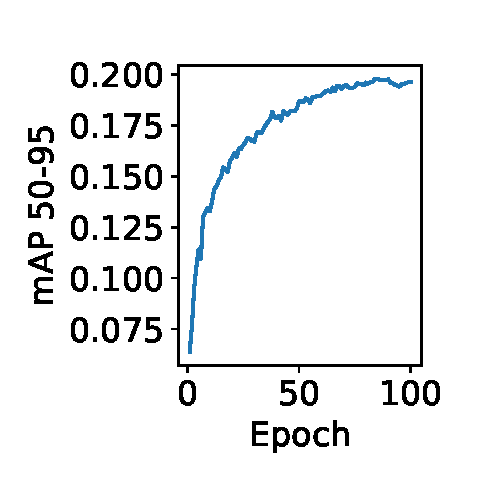
\includegraphics[width=1\linewidth]{images/mAP50-95.eps}
    \end{subfigure}
    \caption{mAP@50 and mAP@50-95 evolution during YOLOv8 training.}
    \label{mAPssistema}
\end{figure}

\begin{figure}[!t]
    \centering
    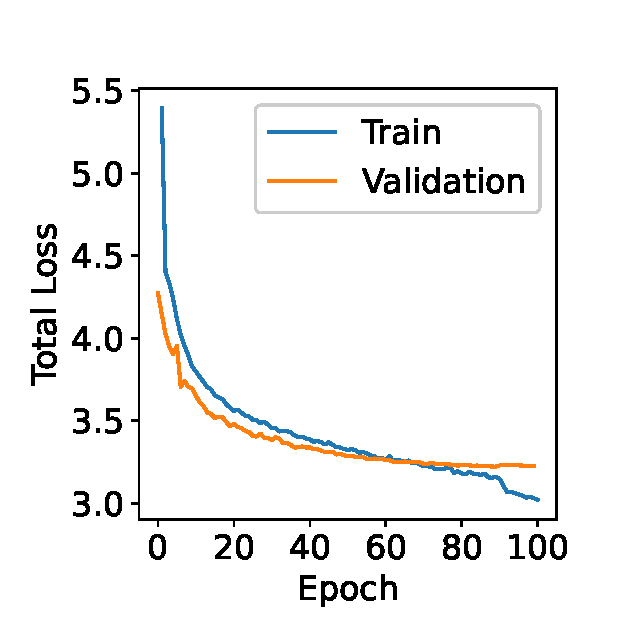
\includegraphics[width=0.5\columnwidth]{images/loss.eps}
    \caption{Loss function convergence during training.}
    \label{Lossfcn}
\end{figure}

A critical factor influencing detection accuracy is the dataset imbalance. As detailed in Table~\ref{Breakdown mAP}, the class ``Car'' achieved a significantly higher mAP@50 ($0.756$) compared to other classes such as ``Bicycle'' ($0.0804$) or ``Awning-tricycle'' ($0.127$). This disparity is primarily due to the overwhelming number of ``Car'' instances in the training set compared to underrepresented classes. 

\begin{table}[!b]
    \caption{mAP@50 and mAP@50-95 Breakdown by Class.}
    \label{Breakdown mAP}
    \centering
    \begin{tabular}{|c|c|c|} 
        \hline
        \textbf{Class} & \textbf{mAP@50} & \textbf{mAP@50-95} \\ [0.5ex] 
        \hline\hline
        Car & 0.756 & 0.519 \\
        \hline
        Bus & 0.503 & 0.354 \\
        \hline
        Van & 0.384 & 0.266 \\
        \hline
        Motor & 0.369 & 0.153 \\
        \hline
        Pedestrian & 0.339 & 0.150 \\ 
        \hline
        Truck & 0.301 & 0.202 \\
        \hline
        People & 0.286 & 0.104 \\
        \hline
        Tricycle & 0.229 & 0.122 \\
        \hline
        Awning-tricycle & 0.127 & 0.081 \\
        \hline
        Bicycle & 0.080 & 0.033 \\
        \hline
    \end{tabular}
\end{table}

For the control system, this implies that tracking performance will vary depending on the target object. A ``Car'' target provides a consistent and reliable signal, whereas a ``Bicycle'' target may result in intermittent detection, introducing noise and potential loss of lock. However, the use of the Kalman Filter effectively mitigates these discontinuities by predicting the state during detection gaps.

\subsection{Latency Characterization}
In networked control systems, precise timing is critical. Following the methodology proposed by Kiesel et al. \cite{KIESEL2022238}, the application-perceived latency $\Delta \tau_{l,\text{application}}$ was rigorously modeled as the sum of temporal delays in the loop:
\begin{equation}
    \Delta \tau_{l,\text{application}} = \tau_{\text{sensor}} + \tau_{\text{controller}} + \tau_{\text{actuator}} + \tau_{\text{network}}.
\end{equation}
where $\tau_{\text{sensor}}$ is the time between an event being sensed and recorded, and $\tau_{\text{network}}$ is the transmission time.

To quantify these values, an empirical test was conducted where an object was instantaneously generated in the simulation frame after 10 seconds. The system took approximately $84 \text{ ms}$ to register the object's position. Given that the YOLOv8 algorithm has an average processing time of $60 \text{ ms}$ ($\tau_{\text{sensor}}$), the remaining $24 \text{ ms}$ is attributed to the UDP network transmission ($\tau_{\text{network}}$). The combined delay of the controller and actuator was fixed at $40 \text{ ms}$ based on the Padé model. Thus, the total latency handled by the control loop is:
\begin{equation}
    \Delta \tau_{l,\text{application}} \approx 60 + 40 + 24 = 124 \text{ ms}.
\end{equation}
This significant delay necessitates a robust control strategy, as latencies of this magnitude can easily destabilize high-gain feedback loops.

\subsection{Gimbal Tracking Response}
The closed-loop performance was evaluated using a step response test. The target object was introduced at $t=10 \text{ s}$ with a non-zero angular offset, forcing the system to react and recenter the gimbal. Fig.~\ref{Step response elevation} illustrates the angular displacement response for both the Elevation and Azimuth axes.

\begin{figure}[!t]
    \centering
    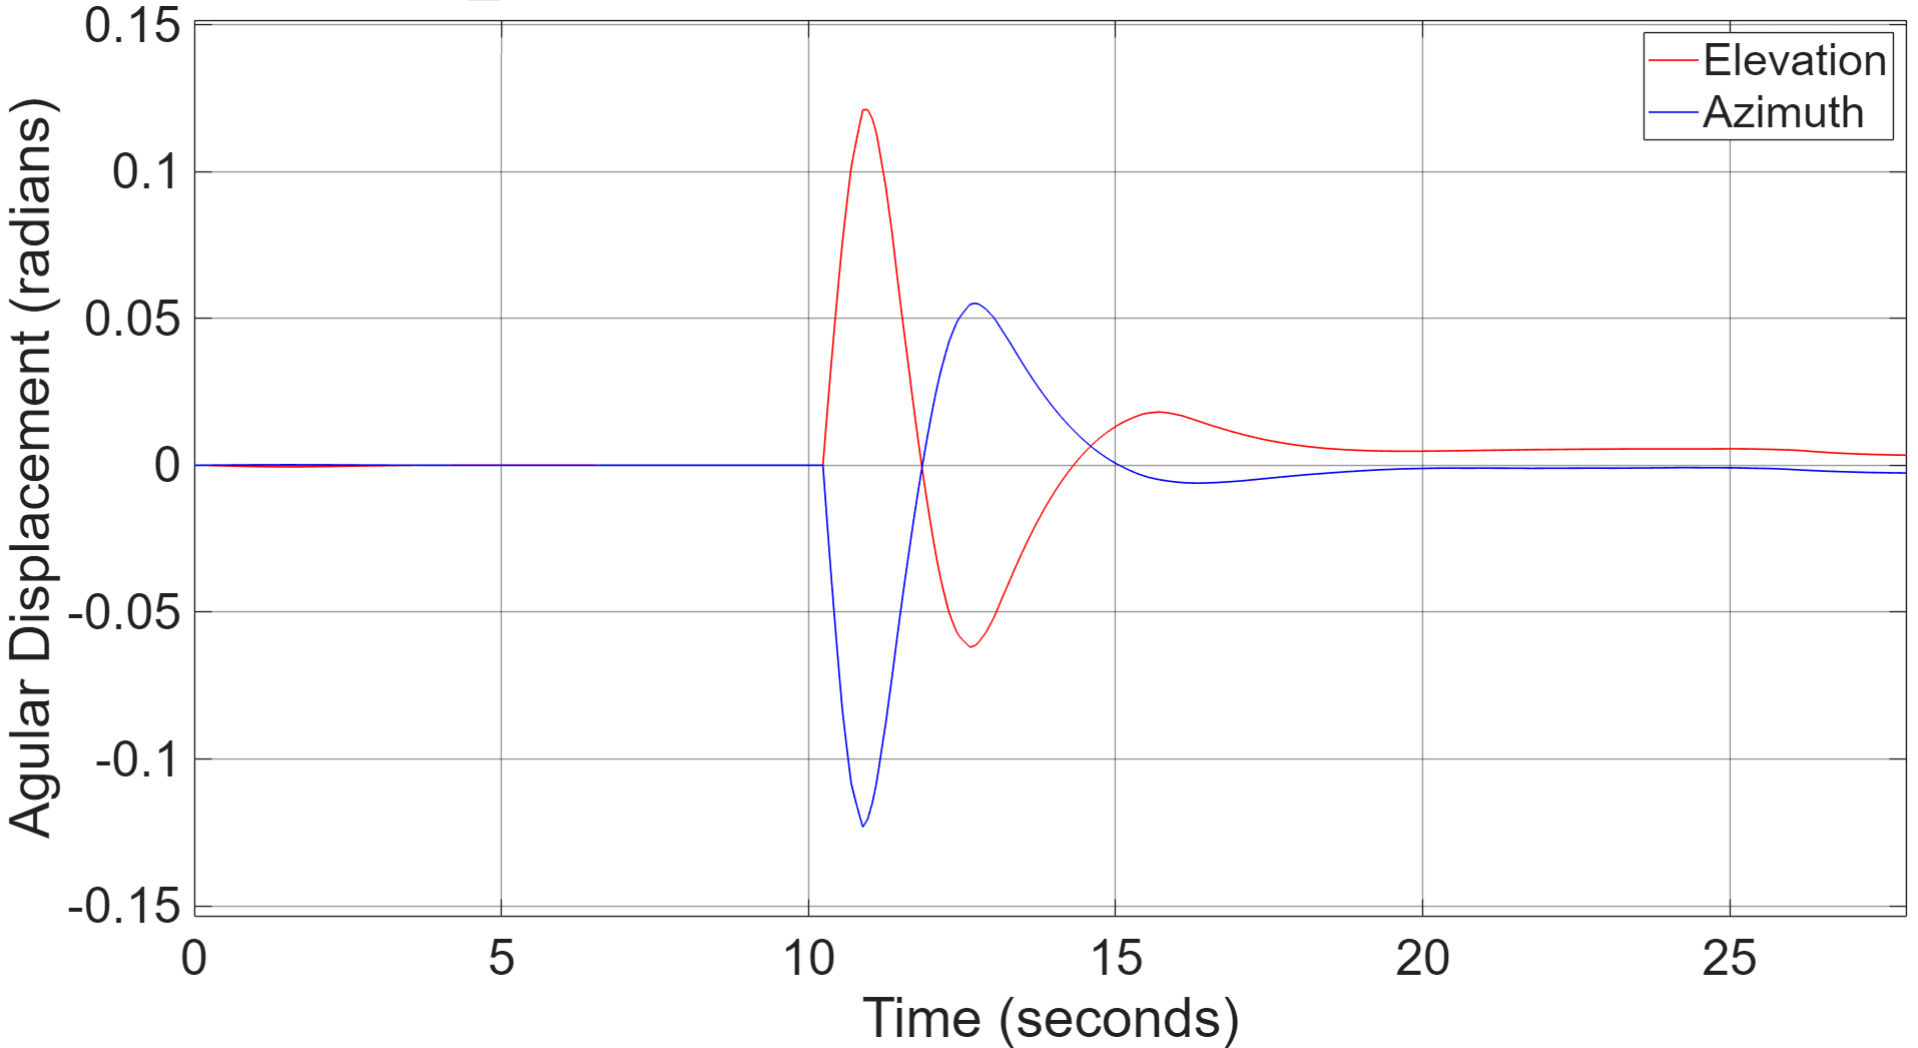
\includegraphics[width=0.9\columnwidth]{images/system_behavior.png}
    \caption{System response to a step input (angular displacement converges to zero).} 
    \label{Step response elevation}
\end{figure}

The results indicate that both axes are stable and successfully converge the angular error to zero. The response is characterized by an initial overshoot, which is expected given the $124 \text{ ms}$ time delay and the aggressive proportional gains used to ensure fast tracking. The Elevation axis exhibits a classic underdamped behavior with a settling time of approximately $5 \text{ seconds}$. 

Interestingly, the Azimuth axis demonstrates a slightly different dynamic profile. While it achieves a comparable settling time, it presents a more oscillatory behavior. This is consistent with the simplified modeling assumption where cross-coupling was neglected; in reality, the inertia seen by the Azimuth axis varies with the Elevation angle, and the fixed PID gains may be slightly less optimal for this axis compared to Elevation.

Fig.~\ref{Torquemotores} presents the control effort required during the maneuver. Crucially, the torque demanded by the PID controller remains well below the motor's saturation limit (stall torque of $6.92 \text{ mNm}$) throughout the transient phase. This validates the physical feasibility of the proposed control law and confirms that the simulation remains within the linear operating region of the actuators. Consequently, complex anti-windup schemes, while beneficial for safety, were not strictly necessary for stability in this nominal operation scenario.

\begin{figure}[!b]
    \centering
    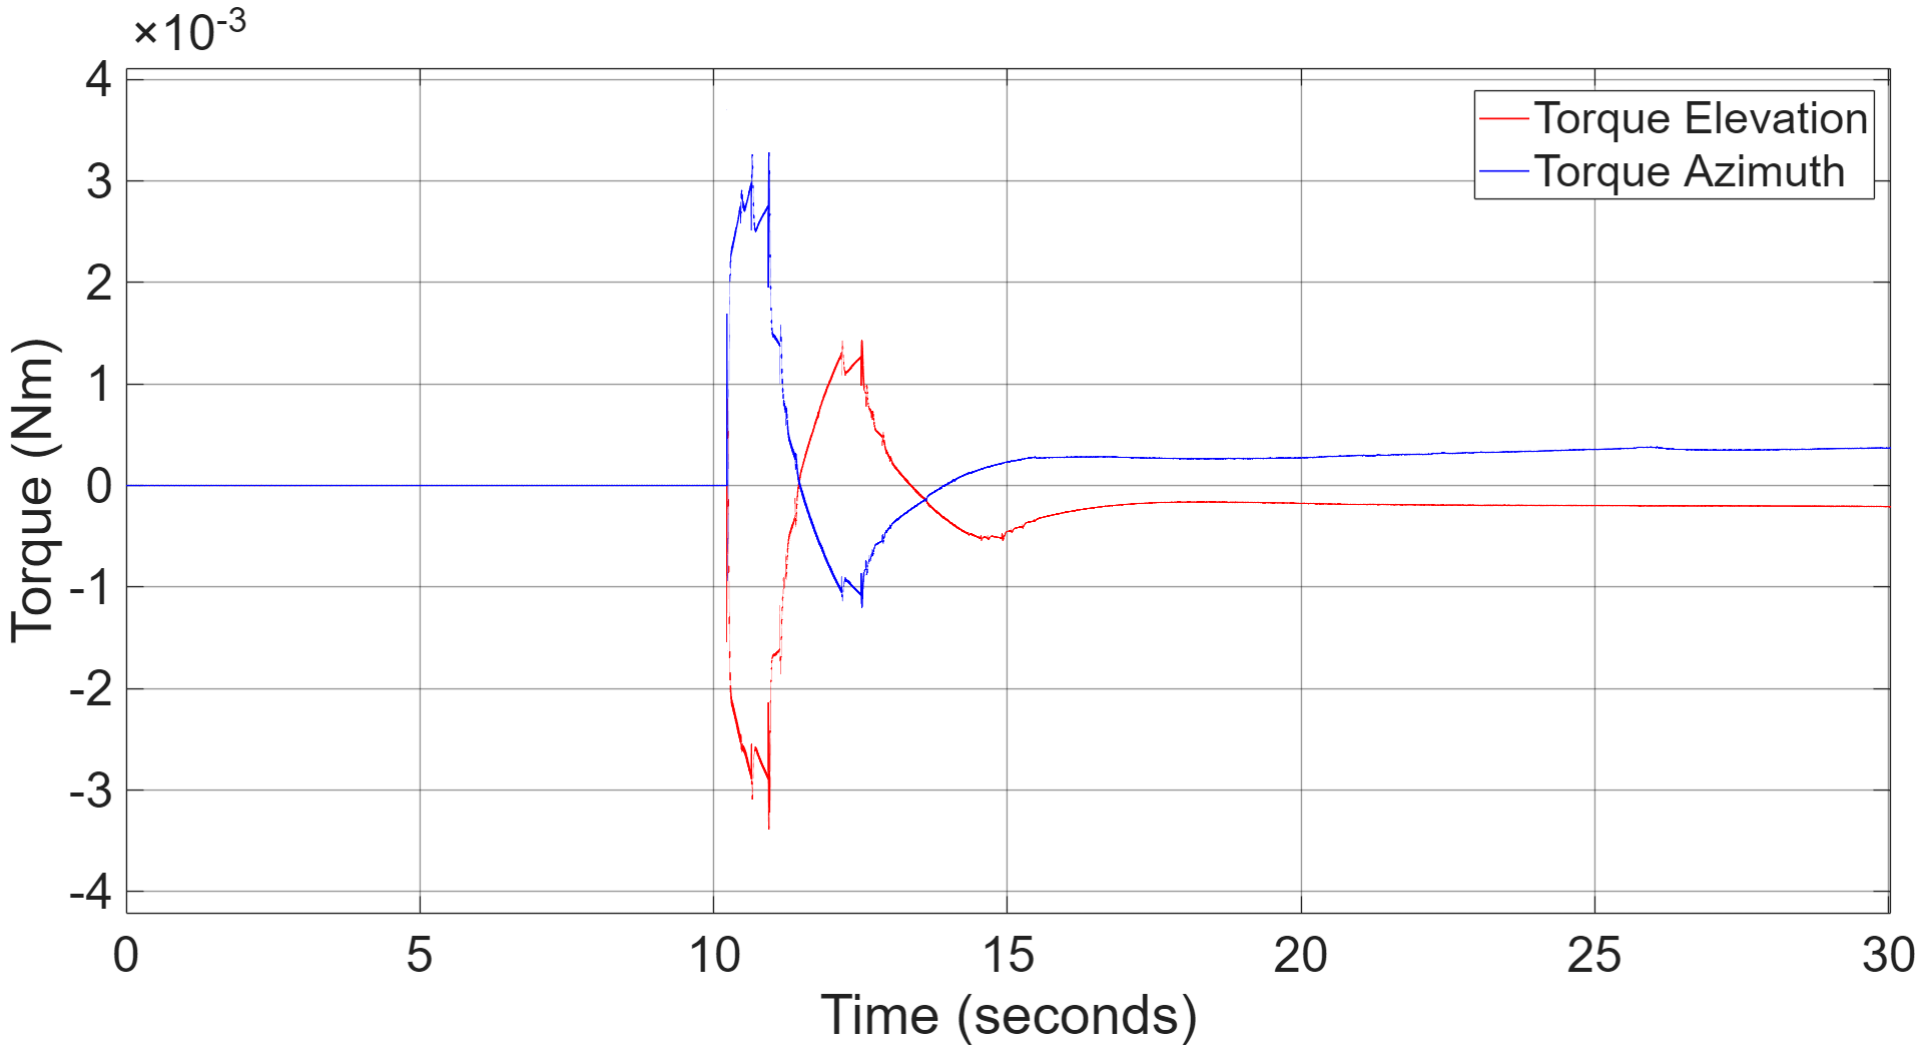
\includegraphics[width=0.8\columnwidth]{images/Torque.png}
    \caption{Torque provided by each electrical DC motor.} 
    \label{Torquemotores}
\end{figure}

The successful tracking of the zero reference demonstrates that the integrated architecture combining vision data, Kalman filtering, and PID control with delay is viable for real-time applications.

\section{CONCLUSION}

This work successfully developed and validated a comprehensive control solution for real-time image-based object tracking utilizing a 2-DOF gimbal. The study addressed the inherent gap between simplified theoretical models and the complexity of real-world mechatronic systems by proposing an integrated architecture that rigorously modeled critical nonlinearities, such as Coulomb friction, and the significant communication delays intrinsic to distributed vision systems.

The core achievement was the seamless integration of a state-of-the-art detector (YOLOv8), a smoothing state estimator (Kalman Filter), and a classical PID controller. Validation in a real-time simulation environment proved that the system could tolerate a total application latency of $124 \text{ ms}$ while maintaining stability. The controller demonstrated responsiveness with a settling time of $5 \text{ seconds}$, effectively centering the target in the field of view. The analysis of torque requirements further confirmed that the proposed solution is physically realizable with standard commercial micro-motors.

Building upon these findings, several avenues for future research are identified to enhance performance and robustness:

\emph{Advanced Control Strategies:} The current PID approach, while stable, exhibits overshoot and oscillation due to the unmodeled dynamics and friction. Investigating advanced nonlinear techniques, such as Sliding Mode Control (SMC) \cite{Rahmat2016Sliding}, is a promising direction. SMC is inherently robust to parameter variations and can handle nonlinear friction more effectively than linear controllers. Alternatively, adaptive algorithms like Fuzzy Logic Control \cite{Galal2009Fuzzy} could allow the system to tune gains in real-time, adapting to changing payloads or inertias.

\emph{Model Refinement and Validation:} The current model assumes a fixed base. Integrating the dynamic angular motion of the base (e.g., aircraft maneuvers) \cite{boiffier1998dynamics} would significantly increase realism for UAV applications. Furthermore, transitioning from pure simulation to Hardware-in-the-Loop (HIL) testing or a physical prototype is the essential next step to validate the latency measurements and control robustness under real-world noise conditions.

\emph{System Optimization:} Finally, the trade-off between detection speed and accuracy remains a bottleneck. Implementing optimization algorithms to auto-tune the PID and Kalman filter parameters could reduce the settling time. Additionally, addressing the dataset imbalance in YOLO training through resampling techniques or data augmentation could significantly improve tracking reliability for non-car objects.

% Acknowledgment (se necessário, remova o comentário)
%\section*{ACKNOWLEDGMENT}


\bibliography{referencias}

% Conteúdo do arquivo referencias.bib (copiado abaixo para fins de submissão em um único arquivo)
% Recomenda-se que você tenha seu .bib separado e use o comando \bibliography{referencias}
% Mas, se for necessário ter tudo junto, você pode colar o conteúdo do .bib aqui, removendo a linha de cima e usando o ambiente thebibliography

% % % Início do Conteúdo BibTeX (para submissão de arquivo único) % % %
% \begin{thebibliography}{00}
% @inproceedings{Mane, ...}
% ...
% \end{thebibliography}
% % % Fim do Conteúdo BibTeX % % %

\end{document}